\documentclass[border=10pt]{standalone}
\usepackage[svgnames]{xcolor}
\usepackage{amsmath}
\usepackage{pgfplots}
\pgfplotsset{compat=newest}
\usepackage[sfdefault]{FiraSans}
\usepackage{FiraMono}
\renewcommand*\familydefault{\sfdefault}
\begin{document}
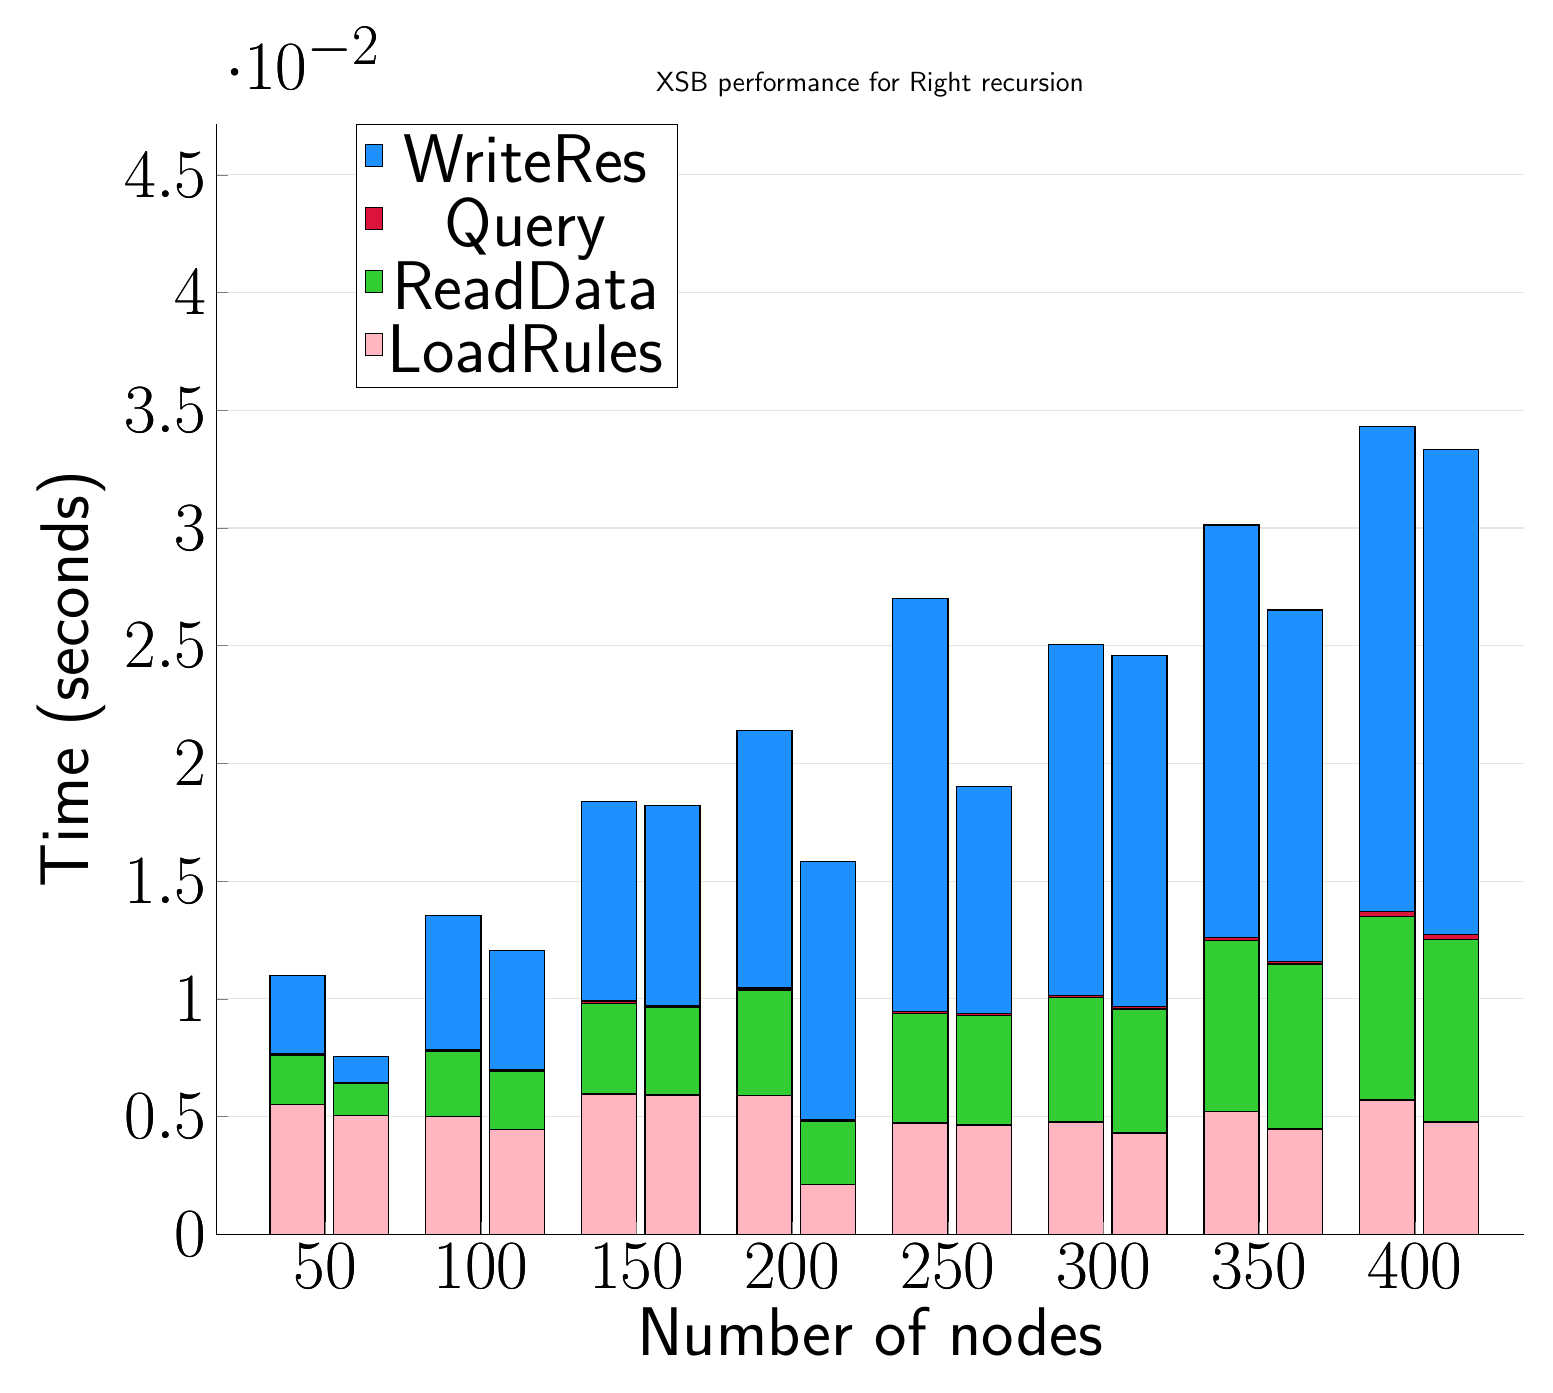
\begin{tikzpicture}
\begin{axis}[
   ybar stacked,
   title={XSB performance for Right recursion},
   bar shift=-10pt,
   width=1.5\textwidth,
   bar width=0.7cm,
   ymajorgrids, tick align=inside,
   major grid style={draw=gray!20},
   xtick=data,
   ymin=0, ymax=0.04718456586201984,
   axis x line*=bottom,
   axis y line*=left,
   enlarge x limits=0.1,
   legend style={
       at={(0.23, 1)},
       anchor=north,
       legend columns=1,
       font=\Huge,
   },
   ylabel={Time (seconds)},
   xlabel={Number of nodes},
   label style={font=\Huge},
   tick label style={font=\Huge},
]
\addlegendimage{fill=DodgerBlue, draw=black, line width=0.2pt}
\addlegendentry{WriteRes}
\addlegendimage{fill=Crimson, draw=black, line width=0.2pt}
\addlegendentry{Query}
\addlegendimage{fill=LimeGreen, draw=black, line width=0.2pt}
\addlegendentry{ReadData}
\addlegendimage{fill=LightPink, draw=black, line width=0.2pt}
\addlegendentry{LoadRules}
\addplot +[fill=LightPink, draw=black, line width=0.5pt] coordinates {
    (50, 0.0055133501688639334)
    (100, 0.004997730255126953)
    (150, 0.00595839818318685)
    (200, 0.005881627400716144)
    (250, 0.004730939865112307)
    (300, 0.0047653516133626264)
    (350, 0.005215724309285484)
    (400, 0.00570201873779297)
};
\addplot +[fill=LimeGreen, draw=black, line width=0.5pt] coordinates {
    (50, 0.00210428237915039)
    (100, 0.00277558962504069)
    (150, 0.0038536389668782536)
    (200, 0.0044910113016764334)
    (250, 0.004644076029459633)
    (300, 0.00528264045715332)
    (350, 0.007254282633463543)
    (400, 0.00779533386230469)
};
\addplot +[fill=Crimson, draw=black, line width=0.5pt] coordinates {
    (50, 4.267692565917967e-05)
    (100, 5.698204040527347e-05)
    (150, 8.734067281087234e-05)
    (200, 8.138020833333337e-05)
    (250, 8.559226989746094e-05)
    (300, 9.69568888346354e-05)
    (350, 0.00012660026550292966)
    (400, 0.00021092096964518234)
};
\addplot +[fill=DodgerBlue, draw=black, line width=0.5pt] coordinates {
    (50, 0.003336588541666664)
    (100, 0.00571934382120768)
    (150, 0.008481661478678392)
    (200, 0.010956605275472034)
    (250, 0.017534097035725938)
    (300, 0.014918724695841464)
    (350, 0.01752408345540367)
    (400, 0.020601669947306285)
};
\end{axis}
\begin{axis}[
   ybar stacked,
   bar shift=13pt,
   width=1.5\textwidth,
   bar width=0.7cm,
   ymajorgrids, tick align=inside,
   major grid style={draw=none},
   xtick=data,
   ymin=0, ymax=0.04718456586201984,
   axis x line*=none,
   axis y line*=none,
   enlarge x limits=0.1,
   label style={font=\Huge},
   tick label style={font=\Huge},
]
\addplot +[fill=LightPink, draw=black, line width=0.5pt] coordinates {
    (50, 0.005040666666666666)
    (100, 0.0044600000000000065)
    (150, 0.005910000000000003)
    (200, 0.0021236666666666635)
    (250, 0.004640666666666667)
    (300, 0.0043033333333333335)
    (350, 0.004474)
    (400, 0.004767666666666663)
};
\addplot +[fill=LimeGreen, draw=black, line width=0.5pt] coordinates {
    (50, 0.0013540000000000004)
    (100, 0.0024589999999999963)
    (150, 0.0037409999999999965)
    (200, 0.0026826666666666696)
    (250, 0.004645666666666667)
    (300, 0.005266333333333341)
    (350, 0.006998999999999997)
    (400, 0.007763)
};
\addplot +[fill=Crimson, draw=black, line width=0.5pt] coordinates {
    (50, 2.733333333333293e-05)
    (100, 5.033333333332817e-05)
    (150, 6.99999999999983e-05)
    (200, 6.266666666666686e-05)
    (250, 8.43333333333321e-05)
    (300, 9.633333333333256e-05)
    (350, 0.0001076666666666702)
    (400, 0.00020833333333333335)
};
\addplot +[fill=DodgerBlue, draw=black, line width=0.5pt] coordinates {
    (50, 0.0011273333333333337)
    (100, 0.005091000000000005)
    (150, 0.008500333333333335)
    (200, 0.010977)
    (250, 0.009643)
    (300, 0.014909)
    (350, 0.01493133333333333)
    (400, 0.020601666666666667)
};
\end{axis}
\end{tikzpicture}

\end{document}
